        \clearpage
        \begin{figure*}[ht]
            \pdfbookmark[2]{ID 03}{figure_id_03}
        	\centering
            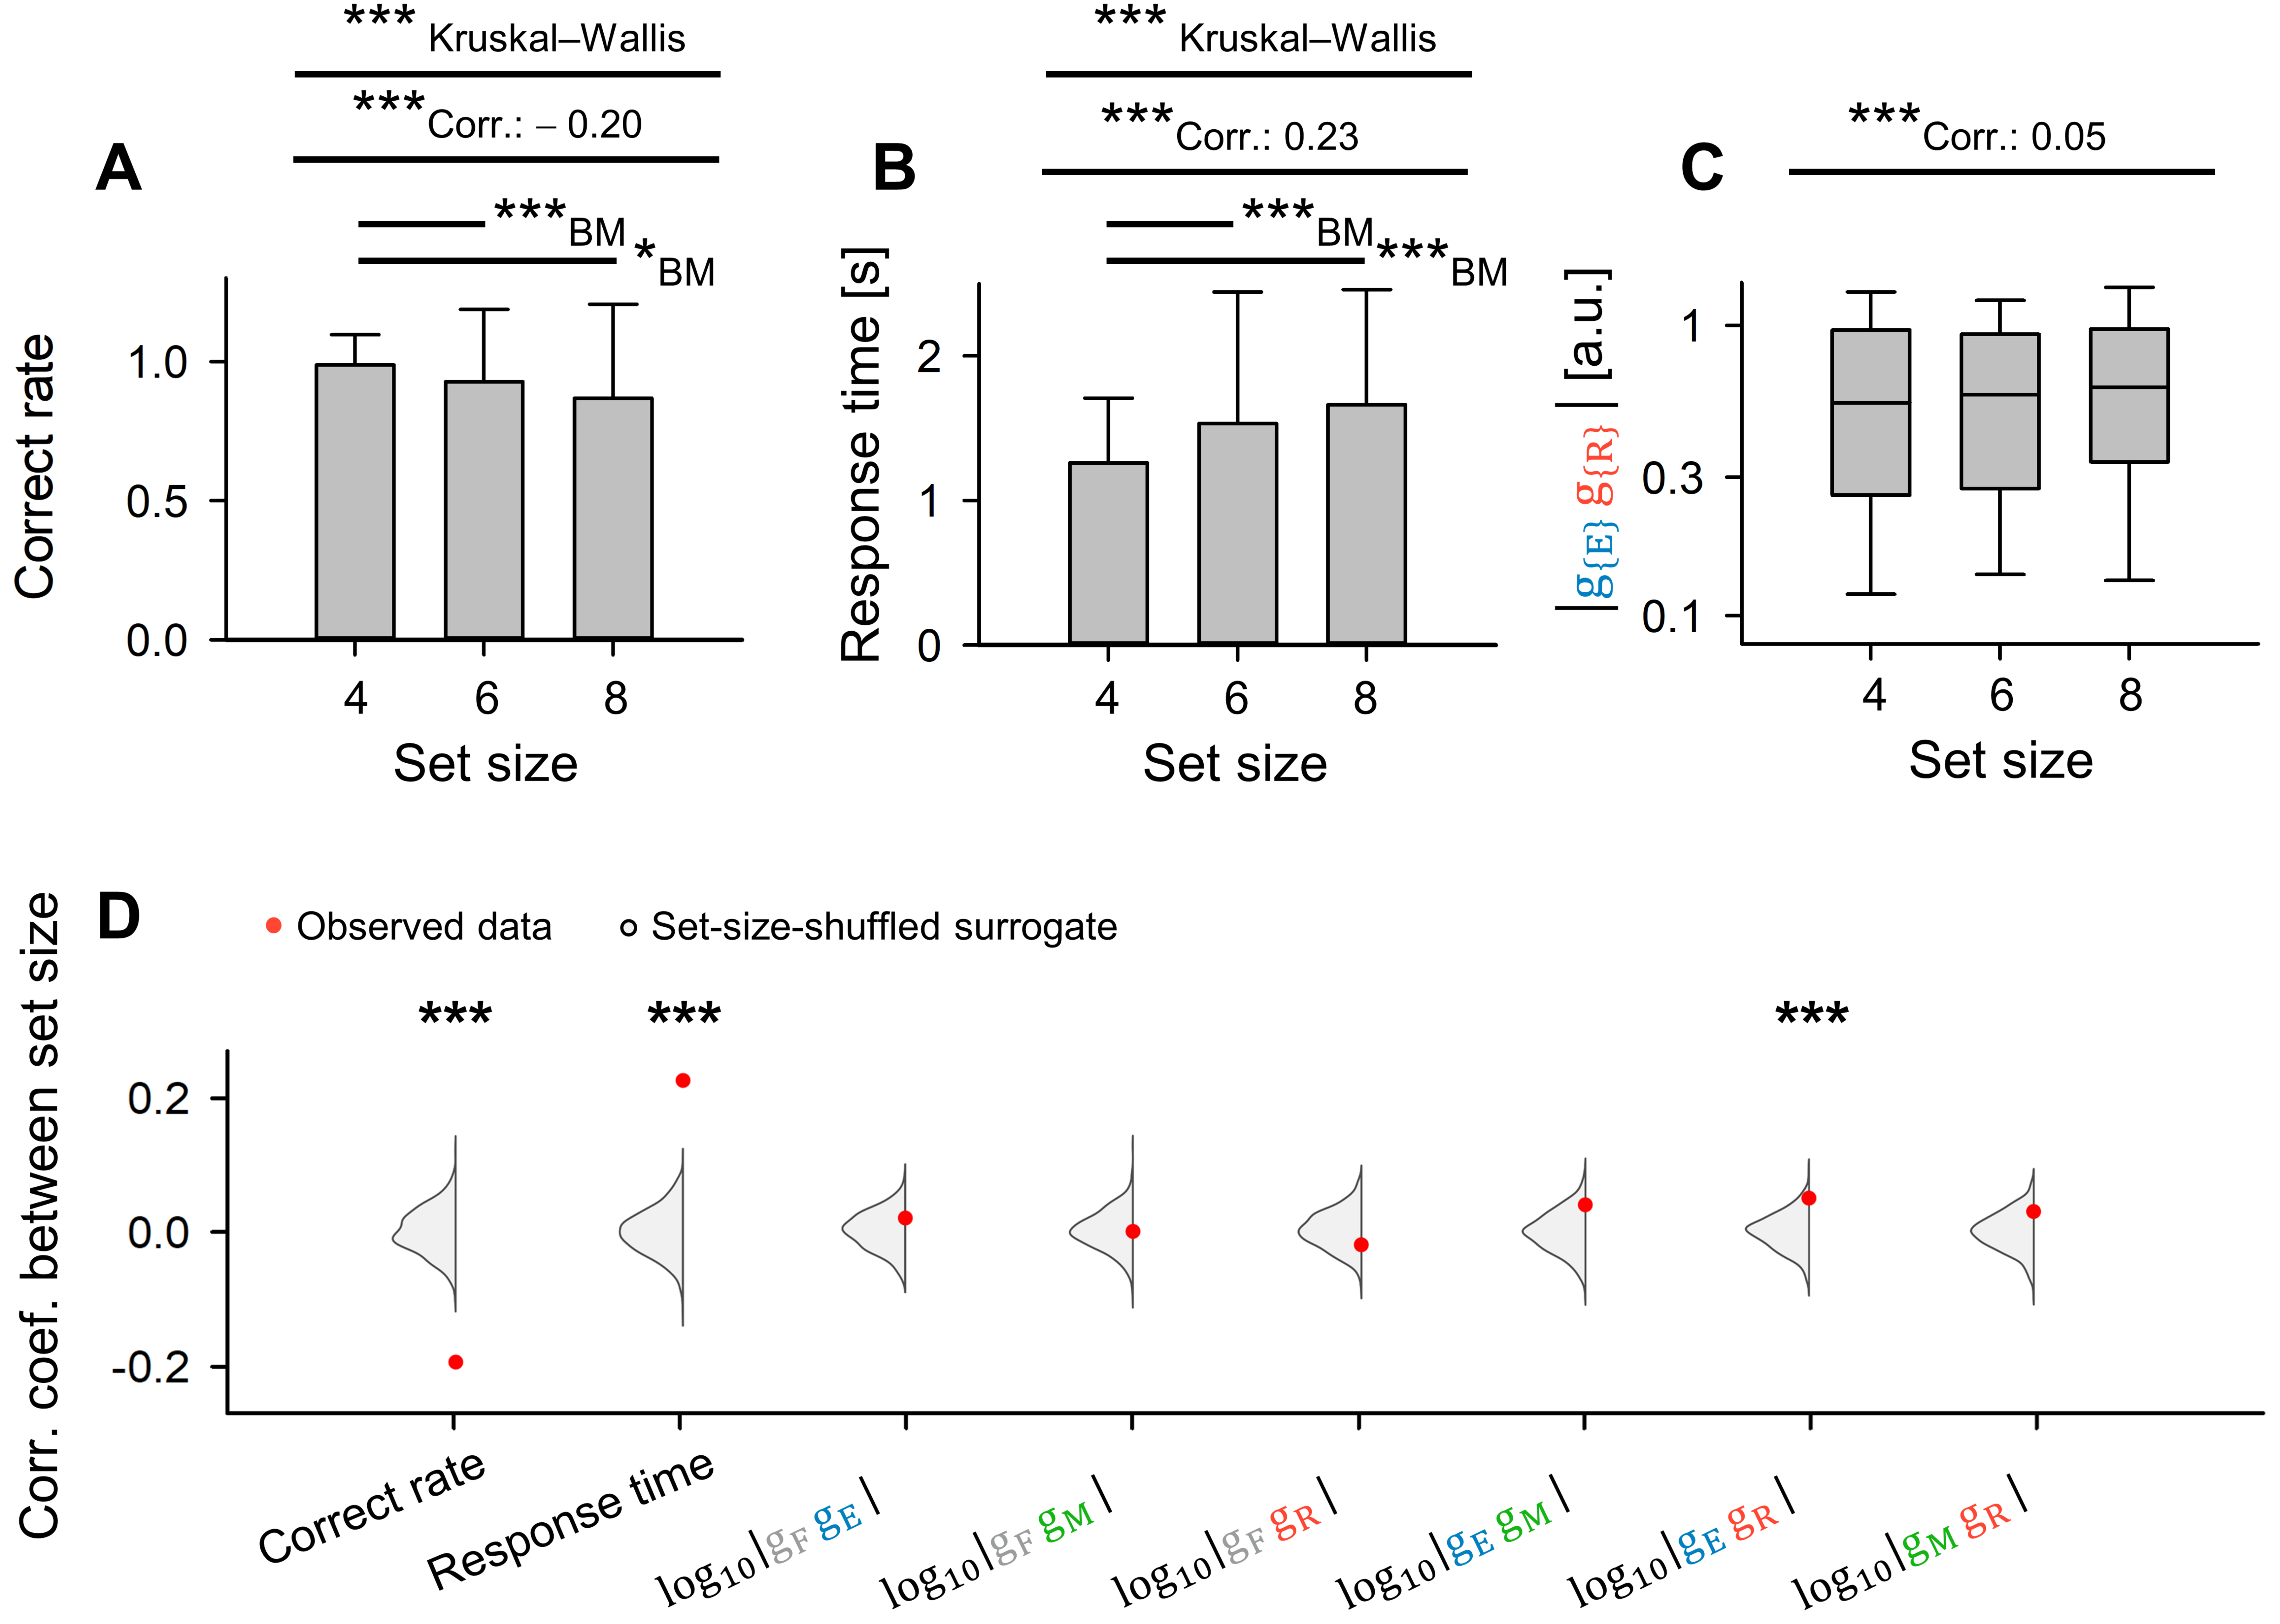
\includegraphics[width=1\textwidth]{./src/figures/.png/Figure_ID_03.png}
        	\caption{\textbf{
Dependence of Trajectory Distance on Memory Load Between Encoding and Retrieval States in the Hippocampus
}
\smallskip
\\
\textbf{\textit{A.}} A significant correlation has been documented between the set size (the number of letters to encode) and the correctness rate in the WM task (coefficient = $-0.20$, ***\textit{p} $<$ 0.001) \cite{van_vugt_hippocampal_2010, li_functional_2023, borders_hippocampus_2022}. \textbf{\textit{B.}} A notable correlation exists between set size and response time (coefficient = $0.23$, ***\textit{p} $<$ 0.001) \cite{dimakopoulos_information_2022}.  \textbf{\textit{C.}} There is a correlation between set size and the distances between encoding and retrieval phases ($\Vert \mathrm{g_{E}g_{R}} \Vert$), but it's less significant (correlation coefficient = 0.05) \cite{li_functional_2023}. \textbf{\textit{D.}} \textit{Red} dots express the observed correlations between set size and the stated parameters: correct rate, response time, $\log_{10}{\Vert \mathrm{g_{F}g_{E}} \Vert}$, $\log_{10}{\Vert \mathrm{g_{F}g_{M}} \Vert}$, $\log_{10}{\Vert \mathrm{g_{F}g_{R}} \Vert}$, $\log_{10}{\Vert \mathrm{g_{E}g_{M}} \Vert}$, $\log_{10}{\Vert \mathrm{g_{E}g_{R}} \Vert}$, and $\log_{10}{\Vert \mathrm{g_{M}g_{R}} \Vert}$. The \textit{gray} kernel density plot illustrates the corresponding randomized set-size measurements (\textit{n} = 1,000) (***\textit{p}s $<$ 0.001) \cite{norimoto_hippocampal_2018, hajos_input-output_2013}.
}
% width=1\textwidth
        	\label{fig:03}
        \end{figure*}
